\begin{refsection}
In this chapter, the methodology followed for the development of this thesis is going to be carried out. This section is going to be divided in two main parts. The first one, will describe the experimental procedures carried out including the linseed oil oxidation kinetic determination, the silica micro-capsules synthesis, the OS film elaboration and the head-space oxygen concentration evolution test. The second part will refer to the computational procedure followed for the development of the design tool program, this includes the physical model description, the numerical resolution approach, the kinetic parameters adjustment strategy and finally the graphical user interface (GUI) programming. 

\section[Exp.Procedure]{Experimental Procedure}
\subsection{Materials}\label{subsec:materials}
Before describing the procedure followed to synthesize active silica micro-capsules containing linseed oil, as well as describing the active film elaboration methodology it is important to state the materials used in these experimental procedures. The materials used are listed in table \ref{tab:material}

\begin{table}[h]
\centering
\caption{Materials used in the experimental procedure for the synthesis of 2g of micro-capsules and for a 17cmx17cm polymeric film.}
\label{tab:material}
\begin{tabular}{|c|c|}
\hline
Material                        & Quantity (per batch) \\ \hline
Ethanol  Absolute               & 36 mL                \\ \hline
Deionized  Water                & 85.5 mL              \\ \hline
Cetrimonium  Bromide (CTAB)     & 0.48 g               \\ \hline
Linseed  Oil                    & 1.5 mL               \\ \hline
Tetraethylorthosilicate  (TEOS) & 6 mL                 \\ \hline
25\% Ammonia Solution           & 3 mL                 \\ \hline
High Density Polyethylene (HDPE) Homopolymer & 62 g            \\ \hline
\end{tabular}
\end{table}



\subsection{Silica micro-capsules synthesis}\label{subsec:met.sintesis}
Regarding the microcapsule synthesis, this has been carried out by the CIPP-CIPEM using the sol-gel emulsion templating methodology. This procedure consists of preparing an emulsion in which the disperse phase is the chemical specie that is desired to be encapsulated. In this case, the surfactant or emulsifier will serve as a template where tetraethyl orthosilicate (TEOS) precursor undergoes hydrolysis and condensation reactions to form the silica polymeric microcapsule \cites{Alvarado2020ValidacionesEncapsulados}. To obtain 2.34g of dry product, initially 85.5 mL of water, 0.48g of cetrimonium bromide (CTAB) and 36mL of ethanol are mixed in a 250mL beaker at a speed of 700rpm during 5 minutes. Afterward, 1.5 mL of double-cooked linseed oil is added drop by drop to the previous mix, and immediately after, 6mL of TEOS is slowly added to the beaker, which is left mixing during 5 minutes more. Finally, 3mL of 25\% ammonia solution is added to the beaker to catalyze the reaction, which is left mixing at 700 rpm for 24 hours. The mix obtained is centrifuged at a velocity of 4000 rpm for ten minutes as a result the micro-capsules obtained are separated from the liquid phase of the mix. Next, the solid is dried in a vacuum oven at 70\degree C and a pressure of $-0.06 MPa$ for 4 hours. After that time, the microcapsules are ready to be incorporated into the polymeric film. In figure \ref{fig:capsules}, an image of the product obtained is shown. 


\begin{figure}[h]
    \centering
    \begin{subfigure}[b]{0.48\linewidth}           \centering
        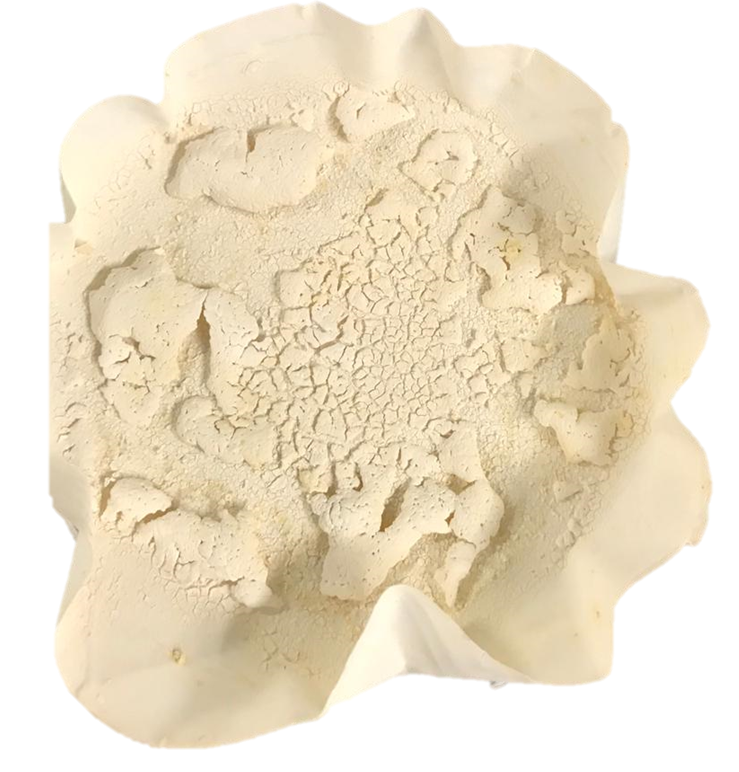
\includegraphics[width=\linewidth]{Documento_Latex/Tesis 2/Imagenes/capsulas (2).png}
    \end{subfigure}
    \begin{subfigure}[b]{0.48\linewidth}
        \centering
        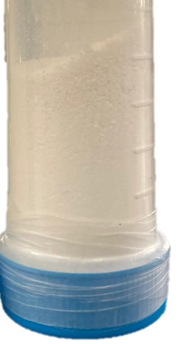
\includegraphics[width=0.5\linewidth]{Documento_Latex/Tesis 2/Imagenes/capsulas.png}
    \end{subfigure}
    \caption{Silica microcapsules obtained by the methodology described in section \ref{subsec:met.sintesis}}
    \label{fig:capsules}
\end{figure}

\subsection{Film Elaboration} \label{sec:film_elaboration}
The film elaboration refers to the the different process which occur between the incorporation of the silica micro-capsules to the final production of polymeric film. Regarding the incorporation of the capsules, once having 9g of this, a masterbatch (MB) is prepared by mixing the micro-capsules load and high density polyethylene (HDPE) homopolymer within an internal mixer, which has to be preheated 10 minutes before at 170\degree C. The ratio of  micro-capsules to HDPE in the mix was 20:80 mass proportion respectively. This mix is poured into the internal mixer for 7 minutes during which the torque and temperature are monitored until this two signals stabilized indicating a homogeneous mixture. The material obtained must was then frozen to a temperature of -80\degree C for 3 hours in an ultra-freezer. This process is necessary to increase the fragility of the material. Afterwards, it was taken into a blade mill for grinding for 1 minute and in this way, the masterbatch (MB) was finished. \\

Next, the masterbatch previously obtained was diluted with HPDE homopolymer to form the films. To do this a mix of 10g of MB and 30g of HPDE was submitted through the same process of mixing as the masterbatch did. Finally, the process of compression molding is done by using a press. To do this, two aluminum foils and two Teflon foils are put over the two sides of the press, and in the inferior part of it, a quantity of 12g of the HDPE-MB mixture is poured using a 17cm x 17cm aluminum frame with a 3cm width. The inferior and superior plates are both preheated to a temperature of 170\degree C and the press must be configured so that an initial pressure of 15 bar is applied during 1 minute and then a pressure of 110 bar must be applied during 1.5 minutes after which a 10 minutes cooling time is done. After this, the desired film of 17cm x 17cm with OS load is obtained (Figure \ref{fig:film}).

\begin{figure}[ht]
    \centering
    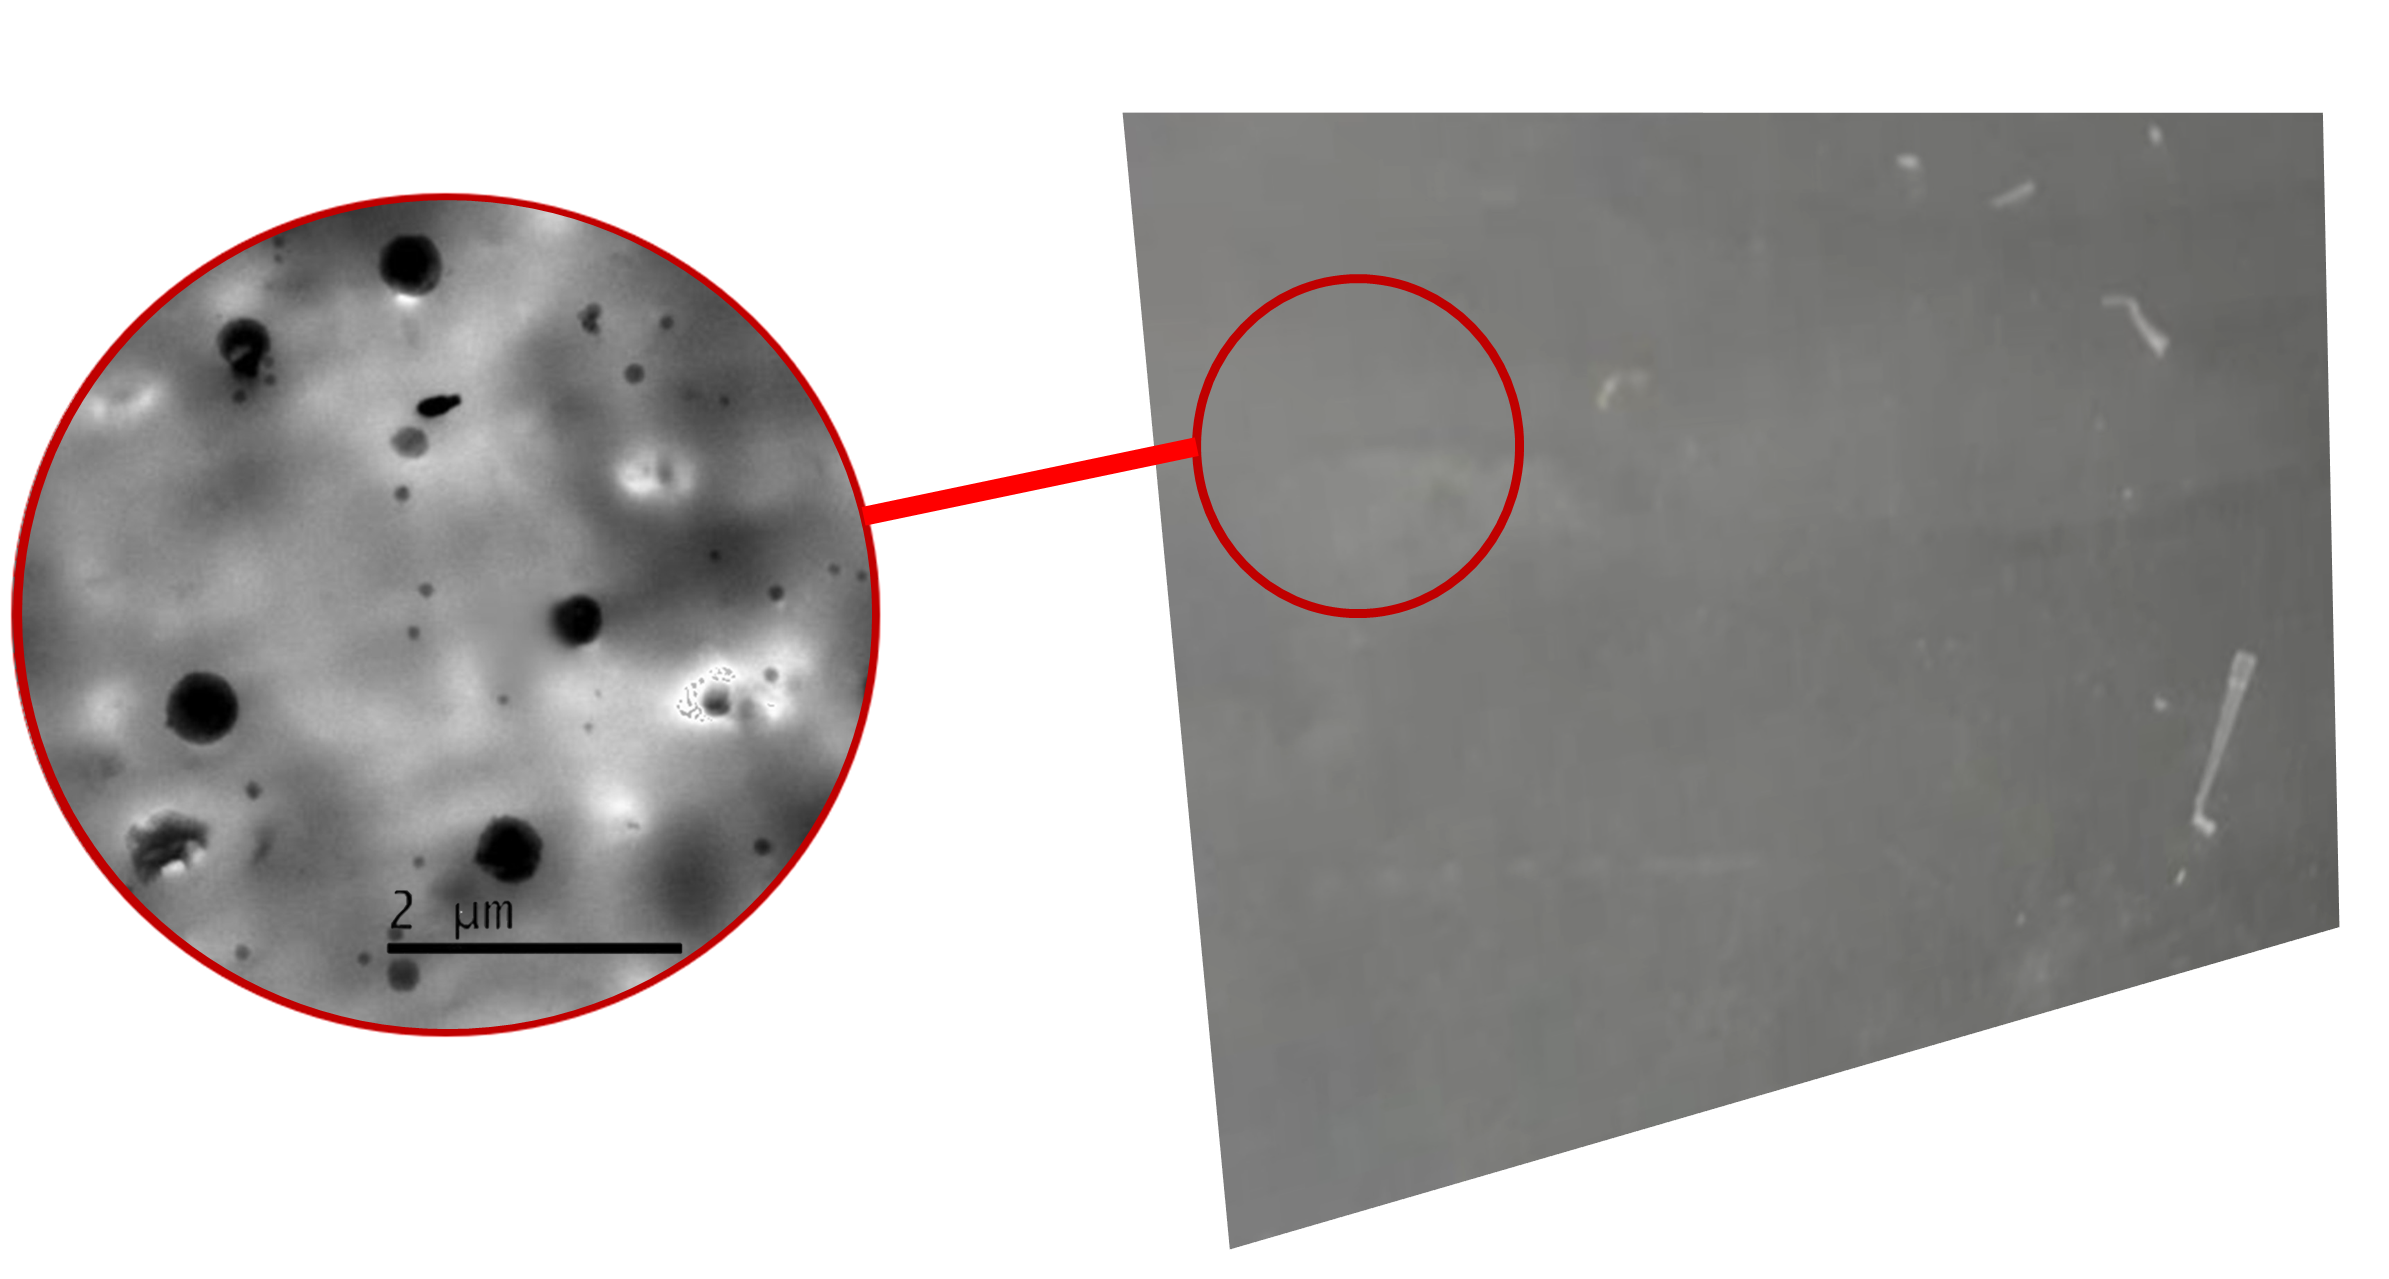
\includegraphics[width=0.6\linewidth]{Imagenes/pelicula.png}
    \caption{HPDE film containing silica microcapsules which were incorporated following the methodology described in section \ref{sec:film_elaboration} \cite{ArellanoAyala2019EfectosAntioxidantes}}
    \label{fig:film}
\end{figure}

\subsection{Headspace Oxygen Absorption Test}\label{sec:headspace}
The head-space is defined in the packaging industry as the volume of gas which is inside a package. In this case the evolution of the oxygen concentration within the head-space gas of a control volume was used as the main experiment to verify the prediction capacity of the physical model and numerical solutions made throughout this thesis. To carry out this test the Quantek Quantek 901 head-space oxygen analyzer was used. This equipment can measure oxygen concentrations going from 0.1\% v/v to 100\%v/v with a 0.1\% v/v precision. The operating principal of the Quantek 901 is based on a fuel cell type oxygen sensor, which consist of a diffusion barrier, a sensing electrode made of platinum and a working electrode made of zinc, all submerged in a solution of potassium hydroxide which acts as an electrolyte \cite{Boissevain1996CorporateGuide}. The entering oxygen diffuses into the sensor and reduces to hydroxyl ions at the cathode, as shown in reaction \ref{reacc:head_spc_1} \reaction[reacc:head_spc_1]{O2 +2H2O +4e^- -> 4OH^-\text{.}} Next, the hydroxyl ions formed are oxidized at the zinc anode (reaction \ref{reacc:head_spc_2}) .
 \reaction[reacc:head_spc_2]{2Pb + 4OH^- -> 2PbO +2H2O + 4e^-\text{,}}
 which yields an overall cell reaction as the one shown in reaction \ref{reacc:head_spc_3}.
 \reaction[reacc:head_spc_3]{2Pb + O2 -> 2PbO}

 
 The current generated during this reaction is proportional to the concentration of oxygen present in the medium. With this in mind,  the sensor measures these currents and calculates the quantity of oxygen within a gas sample \cite{GarciaMora2015KineticScavengers, Boissevain1996CorporateGuide}.\\
 
 The head space oxygen analysis was carried out for silica micro-capsules as well as for 5\% OS HPDE films. To carry out this test, 8cm by 18cm triple layer bags (polypropilene, metallic polyester and low density polietylene respectively, see figure \ref{fig:non_sealed_bag}) were used. To test the nanomaterial, 0.6g of it was introduced into the bag, while for testing the films, a sample of 8cm by 14cm was added to the bag. Once the samples which were going to be tested were within the bags, these were sealed using a Sentinel Heat Sealer 12AS from Packaging Industries Inc., as shown in figure \ref{fig:sealer}. This equipment was preheated to a temperature of 400\degree C and the bags  were pressed within the sealer during 4 seconds, after which the bag was sealed as shown in figure \ref{fig:sealed_bag}.  
 
 \begin{figure}[h]
    \centering
    \begin{subfigure}[b]{0.3\linewidth}           \centering
        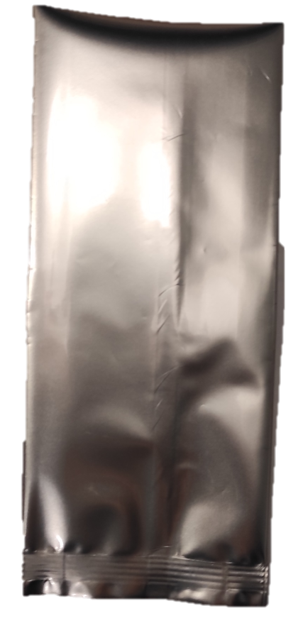
\includegraphics[width=0.5\linewidth]{Documento_Latex/Tesis 2/Imagenes/Non_Sealed_Bag.png}
        \caption{ }
        \label{fig:non_sealed_bag}
    \end{subfigure}
    \begin{subfigure}[b]{0.3\linewidth}
        \centering
        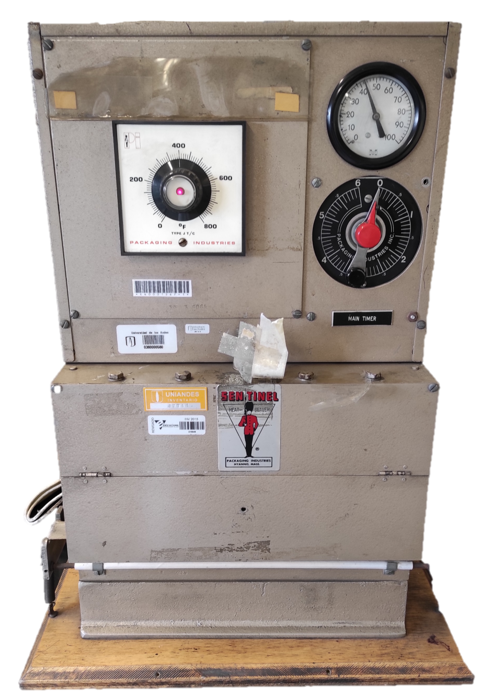
\includegraphics[width=0.8\linewidth]{Documento_Latex/Tesis 2/Imagenes/Sealer.png}
        \caption{ }
        \label{fig:sealer}
    \end{subfigure}
    \begin{subfigure}[b]{0.3\linewidth}
        \centering
        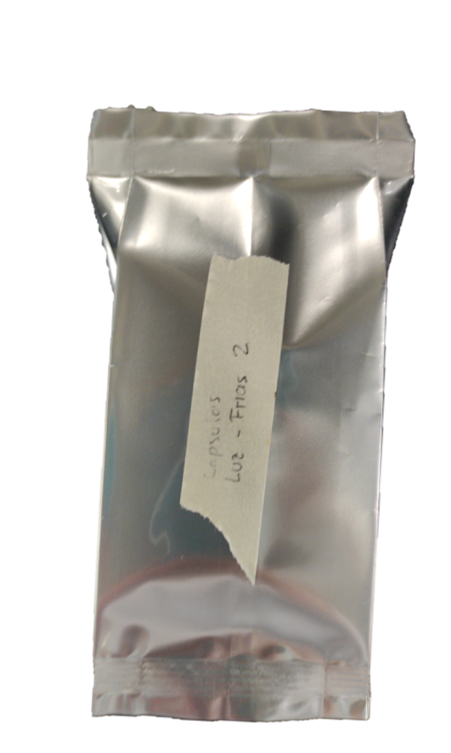
\includegraphics[width=0.8\linewidth]{Documento_Latex/Tesis 2/Imagenes/Sealed_Bag.png}
        \caption{ }
        \label{fig:sealed_bag}
    \end{subfigure}
    \caption{Representation of the bags used for the headspace experiment \textbf{a)} before sealed and \textbf{c)} after sealed,  by using the heat sealer shown in image \textbf{b)}}
    \label{fig:bags}
\end{figure}

Once the bags were sealed, they were filled with 120mL of air. This was done by sticking a adhesive acrylic with polyethylene liner septa to the surface of the bag and injecting through it the desired quantity of air with a graduated syringe. The septa used prevents that air gets into the bag once they are stabbed so the head space atmosphere is only altered by the presence of the capsules or the film within it.

Also, it is important to clarify that the tests for the 1.2g of capsules and the 5\% OS HPDE films were made by triplicate and that a negative control was set by filling three bags with only air, this to monitor that the oxygen concentration within them remains stable throughout the test. \\

Finally, to carry out the headspace oxygen concentration test, a bag must be puncture through the EPDM septa using the needle attached to the Quantek Oxygen Analyser. This equipment was calibrated to take a sample of 2mL of the headspace gas within the test bag, which is analysed by the equipment which finally  reports the oxygen volumetric concentration in headspace gas (See figure \ref{fig:headspace_test_image}). The tests made were of destructive nature, meaning that once a bag was punctured to do a measurement, it was immediately discarded. This approach assumes that the behavior of the oxygen absorption by a sample in each bag is going to be equal in all the bags, and has the advantage (over the non-destructive approach) that it do not allows the leakage of atmospheric oxygen due to successive measurements over the same bag. 


Each measurement was made every 48 hours and a total of 6 data points were taken (which cover up a total time of 340 test hours).

\begin{figure}[h]
    \centering
    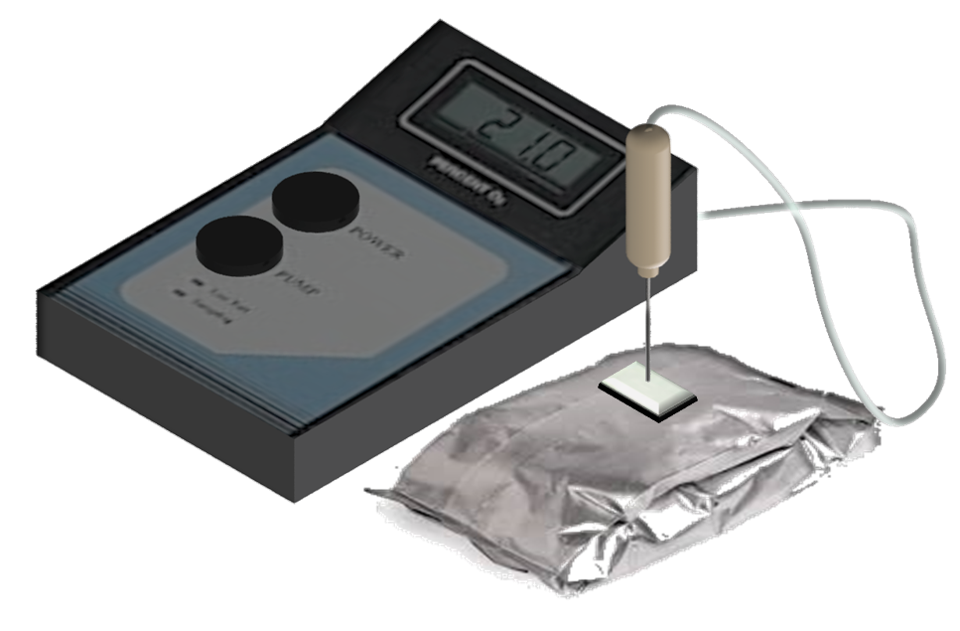
\includegraphics[width=0.7\textwidth]{Documento_Latex/Tesis 2/Imagenes/Headspace_test.png}
    \caption{Representation of the oxygen headspace concentration test assembly.}
    \label{fig:headspace_test_image}
\end{figure}
 
\subsection[Oxidative TGA]{Oxidative Termogravimetric Analysis}\label{sec:TGA} 
To carry on the development of the design tool it is important to determine the oxidation kinetics of double cooked linseed oil. Given that in the autoxidation
process described in Section \textbf{X}, there is an increase in the weight of oils due to the absorption of oxygen from the environment. Even though these changes in weight are minimal, they are big enough for being detected in a thermogravimetric analysis (TGA). So to establish the oil autoxidation reaction constants, TGA test in several atmospheres and temperatures were carried over double cooked linseed oil samples.\\


All tests were made using a simultaneous TGA-DSC SDT Q600 (TA instruments) with a sample of 26mg of linseed oil and using a heating rate of 20\degree C . The different conditions used in every TGA run made is shown in table \ref{tab:TGA_test}

\begin{table}[h]
\centering
\caption{Linseed oil TGA test conditions evaluated to determine the oxidation kinetics constants.}
\label{tab:TGA_test}
\begin{tabular}{|c|c|c|}
\hline
Sample &
  Atmosphere &
  Temperature {[}\degree C{]} \\ \hline
\multirow{9}{*}{\begin{tabular}[c]{@{}c@{}}Linseed Oil\\  (26mg)\end{tabular}} &
  \multirow{3}{*}{Nitrogen UAP} &
  25 \\ \cline{3-3} 
 &                          & 40 \\ \cline{3-3} 
 &                          & 80 \\ \cline{2-3} 
 &
  \multirow{3}{*}{\begin{tabular}[c]{@{}c@{}}Oxygen UAP 70\% v/v - \\ Nitrogen UAP 30\% v/v\end{tabular}} &
  25 \\ \cline{3-3} 
 &                          & 40 \\ \cline{3-3} 
 &                          & 80 \\ \cline{2-3} 
 & \multirow{3}{*}{Dry Air} & 25 \\ \cline{3-3} 
 &                          & 40 \\ \cline{3-3} 
 &                          & 80 \\ \hline
\multicolumn{2}{|c|}{Time per test run {[}h{]}} &
  24 \\ \hline
\end{tabular}
\end{table}


 The rst TGA test carried out was under a nitrogen atmosphere. This is done to
observe the sole eect of the 
ow of air around linseed oil and OS lms. In this case, the
volatile components within the sample are going to evaporate, generating a reduction in
the measured mass. The second TGA test, which has to be carried is in a pure oxygen
atmosphere. This is the case in which oxygen is in excess concerning the substrate, so
the kinetics of oxidation can be simplied, as explained in section 1.2.4. The results in
the change of mass of the sample obtained are normalized for the mass reduction due
to the evaporation obtained from the nitrogen atmosphere TGA. In this way, there is a
guarantee that the changes observed in the mass on the oxygen TGA are exclusively due
to the absorption of oxygen. The third and nal TGA made was in air atmosphere, in
which oxygen has a concentration of 21 vol%. Contrary to the case of oxygen atmosphere
TGA, in this case, it is not correct to assume that oxygen is in excess to the substrate in
the oil, so the results obtained in this test must be compared to the complete autoxidation
kinetics of the linseed oil.
 

 
 
 




\end{refsection}